\newpage
\section{Question 6}
	This section heavily involved MATLAB code. See Appendix A [6] for code listings.
	\subsection{Image Processing}
	\newline The image taken from the camera will be cropped to isolate the working space. As the camera is fixed we can use a constant coordinates for cropping. Then convert the image into double and used adapthisteq to enhance the contrast of the image using histogram equalization. This makes it easier to work on the image as the image was dark and histogram was not equally distributed.  Top faces of the boxes were black. In a grey image which is double 0 is for black and 1 is for white. So we used a threshold of 0.1 to extract top faces from the image. We remove all the areas smaller than 1000 pixels to get rid of noise and used a square structuring element to morphologically close founded areas and fill all holes.\newline

	\subsection{Finding Centroids}
	\newline To find centroids we used regionprops. First we found the coordinates of the fiducial boxes and remove them from the centroid list. (If only the fiducials were present code will give a warning).To match the coordinates with given world coordinate system we used perpendicular distance to the each centroid from the line connecting two fiducial boxes. For example y distance can be found by the perpendicular distance from the line connecting two fiducial boxes which are vertical. \newline
	\pagebreak
	\subsection{Finding Orientation}
	\newline Several methods were tested to find the block orientation, mainly using different sub commands of regionprops. Firstly, we attempted to use the obviously named Orientation command. This met with limited success, as the orientation function works by forming an ellipse around the centroids, and then determining the angle between the major ellipse axis and the horizontal: \newline
	\begin{figure}[position = here]
		\begin{centering}
			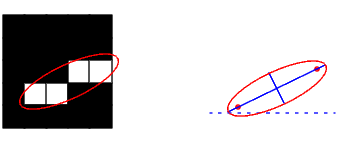
\includegraphics[scale=1]{q6_1}\\
			\caption[\textit{RPYAxes}]{RegionProps Orientation}
		\end{centering}
	\end{figure}
	\newline
	Due to the fact that the identified boxes where not perfectly smooth, this meant that the ellipse major axis did not necessarily run along the boxes diagonal, leading to somewhat erratic angle results.\newline \newline The second method was to instead look at the Extrema of the boxes, as shown below: \newline
	\begin{figure}[position = here]
		\begin{centering}
			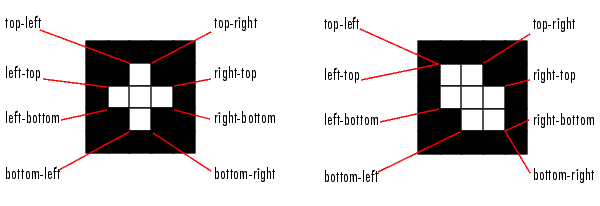
\includegraphics[scale=1]{q6_2}\\
			\caption[\textit{RPYAxes}]{RegionProps Extrema}
		\end{centering}
	\end{figure}
	\newline
	With this, the irregular nature of the boxes is tempered slightly by the eight extreme points, enabling the selection of the longest side and the determining of the angle it made with the horizontal.\newline
	\begin{figure}[position = here]
		\begin{centering}
			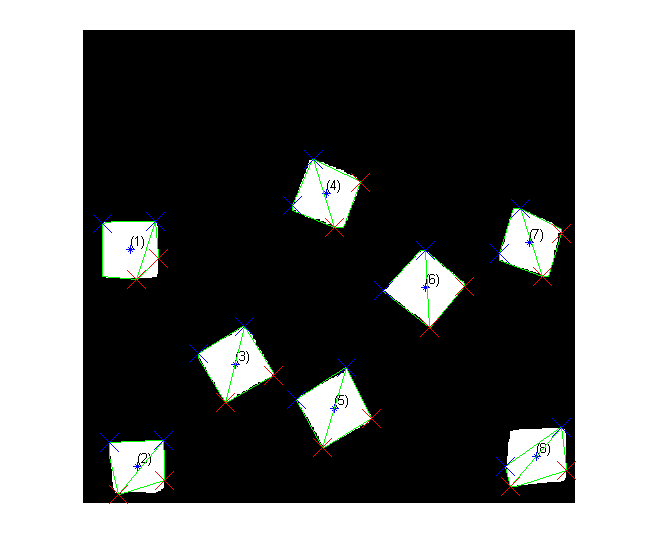
\includegraphics[scale=0.5]{q6_3}\\
			\caption[\textit{RPYAxes}]{RegionProps Extrema in Action}
		\end{centering}
	\end{figure}
	\pagebreak
	\newline
	This method proved simple, yet effective. Though it was not fully implemented, programming the system ti intelligently determine the longest side and determine the angle based on that was considered. However, as can be seen in the above figure, the longest side was not always a side at all. Extremas flaw was that what were determined to be the extreme points were not always the corners, sometimes resulting in diagonals being formed, making strange triangles out of the boxes. The accuracy of the extrema was limited to the clarity of the image, and we had reached the limit of image sharpening using our current techniques - any adjustment of variables resulted in warped boxes.\newline However, it was determined that the inaccuracies in the angle derived from the extrema was within the margin of error acceptable for foam blocks being picked up by a robotic arm.\newline \newline
	
	
	\subsection{Performance}
	\newline
	When our codes was run on the robotic arm, it performed nearly perfectly (after the adjustment of a few unnoticed bugs that prevented operation at all). Unfortunately, when carrying the final block and attempting to stack it, the block was not quite lifted high enough and clipped the tower, knocking it over. Otherwise, the code performed near-perfectly. it correctly identified centroids and orientation for the majority of the blocks, with only a single block having the correct centroids but slightly incorrect orientation. However, this error was within the limits of the arm and foam blocks, and the block was picked up nethertheless.\newline \newline
	
	\subsection*{Code Listing}
	See Appendix A [6] for all code used.

\pagebreak